\documentclass{exam}
\printanswers
\usepackage{times}
\usepackage[T1]{fontenc}
\usepackage[portuges]{babel}


% Comentar para not MAC Users
\usepackage[utf8]{inputenc}

\usepackage{a4}
%\usepackage[margin=3cm,nohead]{geometry}
\usepackage{epstopdf}
\usepackage{graphicx}
\usepackage{fancyvrb}
\usepackage{amsmath}
\usepackage{float}
%\renewcommand{\baselinestretch}{1.5}



\begin{document}
\title{Protocolo IPv4}

\author{Etienne Costa(A76089) \and Joana Cruz(A76270) \and Rafael Alves(A72629)}

\date{}
\maketitle

\begin{abstract}
O principal objectivo deste trabalho é o estudo do Internet Protocol (IP) nas principais vertentes, nomeadamente: estudo do formato de um pacote ou datagrama IP, fragmentação de pacotes IP, endereçamento IP e encaminhamento IP.
\end{abstract}
\section{Parte I}
\subsection{Exercício 1}

\begin{figure}[H]
\centering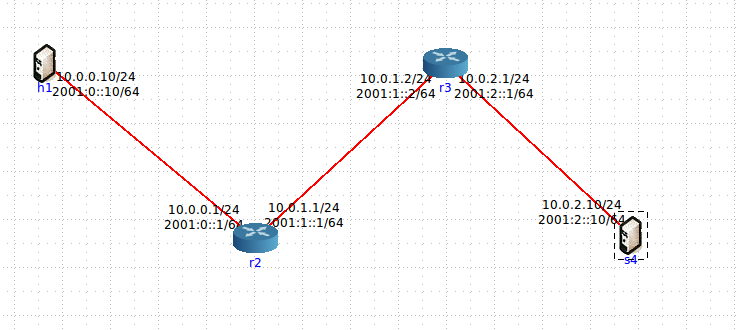
\includegraphics[scale=0.60]{topologia} 
\caption{\label{fig:controller}Topologia Core.}
\end{figure} 

\begin{questions}

\question Active o wireshark ou o tcpdump no pc h1. 
Numa shell de h1, execute o comando traceroute -I para o endereço IP 
do host s4.
\begin{solution}
\begin{figure}[H]
\centering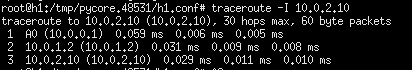
\includegraphics[scale=0.80]{traceroute} 
\caption{\label{fig:controller}Resultado do Traceroute}
\end{figure}
\end{solution}

\question Registe e analise o tráfego ICMP enviado por h1 e o tráfego ICMP recebido como resposta. Comente os resultados face ao comportamento esperado.
\begin{solution}
Inicialmente, o host h1 envia 3 pacotes com o TTL igual a 1 que por sua vez são descartados pelo router r2 pois excedia o TTL. 
De seguida, o TTL é incrementado para 2 e são enviados 3 pacotes que são descartados pelo router r3, 
pois também excedia o TTL. Finalmente, o TTL é incrementado para 3 fazendo com que os pacotes
cheguem até ao host s4, devolvendo uma mensagem (Echo ping) reply.
\begin{figure}[H]
\centering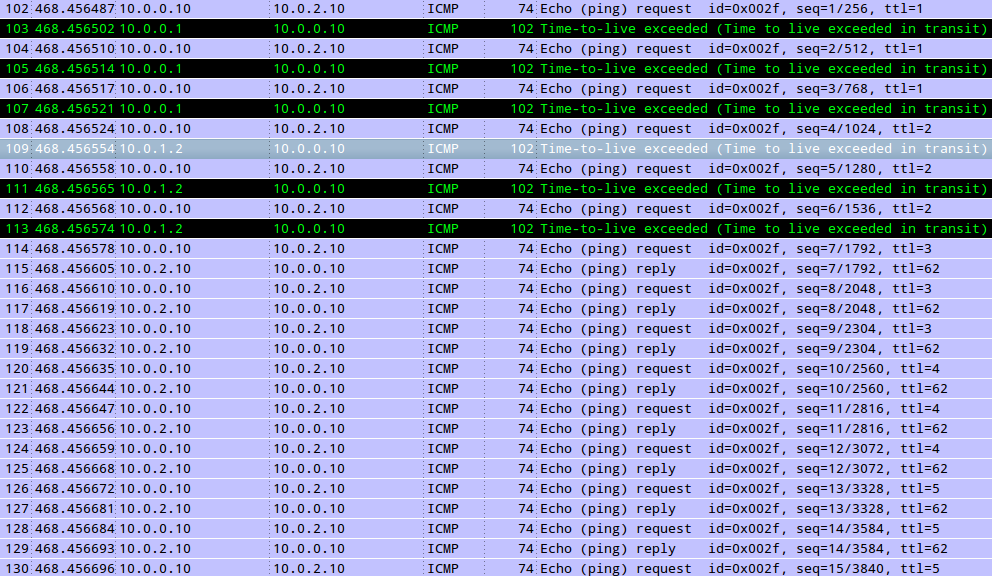
\includegraphics[scale=0.32]{trafegoicmp} 
\caption{\label{fig:controller}Tráfego ICMP}
\end{figure} 
\end{solution}

\question Qual deve ser o valor inicial mínimo do campo TTL para alcancar o destino s4? Verifique na prática que a sua resposta está correta.
\begin{solution}
O valor mínimo que o campo TTL deve ter para alcançar o destino s4 é 3. 
\end{solution}

\question Qual o valor médio do tempo de ida-e-volta (Round-Trip Time) obtido?
\begin{solution}
O valor médio do tempo de ida e volta é 0.017 ms.
\begin{equation}
Round Trip Time= \frac{(0.029 ms + 0.011 ms + 0.010 ms)}{3}
\end{equation}
\end{solution}

\end{questions}

\subsection{Exercício 2}

\begin{questions}

\question  Qual é o endereço IP da interface ativa do seu computador? 
\begin{solution}[.2in]
Tirando partindo do comando ifconfig é possível determinar que o IP da nossa máquina é : 
172.26.64.93.
\begin{figure}[H]
\centering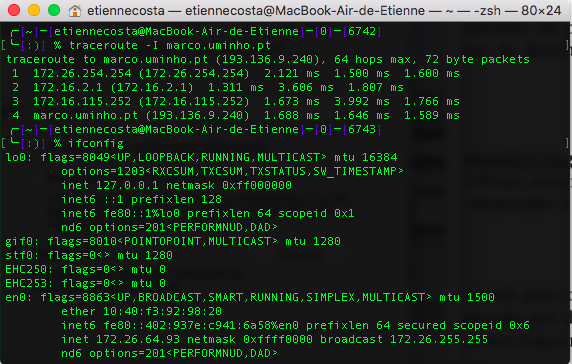
\includegraphics[scale=0.50]{ifconfig} 
\caption{\label{fig:controller}Resultado do ifconfig.}
\end{figure} 
\end{solution}

\question Qual é o valor do campo protocolo? O que identifica?
\begin{solution}[.2in]
O valor do campo protocolo é o ICMP ou seja Internet Control Message Protocol, que é um protocolo utilizado para fornecer 
relatórios de erros à fonte original.
\end{solution}

\question Quantos bytes tem o cabe\c{c}alho IP(v4)? 
Quantos bytes tem o campo de dados (payload) do datagrama? Como se calcula o tamanho do payload?
\begin{solution}[.2in]
O cabeçalho IP possuí 20 bytes.
O campo de dados do datagrama possuí 52 bytes e é calculado através da fórmula abaixo indicada.
\begin{equation}
Payload=Total Length - Header Length
\end{equation}
\begin{figure}[H]
\centering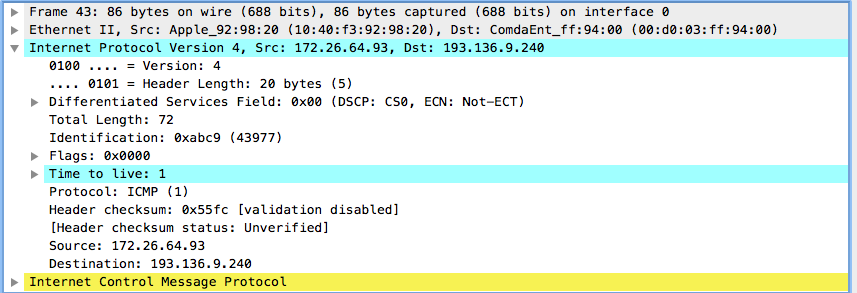
\includegraphics[scale=0.38]{PrimeiraICMP} 
\caption{\label{fig:controller}Primeira mensagem ICMP.}
\end{figure} 
\end{solution}

\question O datagrama IP foi fragmentado? Justifique.
\begin{solutionorlines}[2in]
Não, pois as flags Fragment Offset e More Fragments são iguais a 0.
\end{solutionorlines}

\question Ordene os pacotes capturados de acordo com o endere\c{c}o IP fonte (e.g.,
selecionando o cabe\c{c}alho da coluna Source), e analise a sequência de tráfego ICMP gerado a partir do endere\c{c}o IP atribuído à interface da sua máquina. Para a sequência de mensagens ICMP enviadas pelo seu computador, indique que campos do cabe\c{c}alho IP variam de pacote para pacote.
% Perguntar se é suposto verificar os pacotes na qual a nossa máquina é o destino ou source.
\begin{solution}[2in]
No cabe\c{c}alho IP os campos que variam são: Identification e o Header Checksum.
\begin{figure}[H]
\centering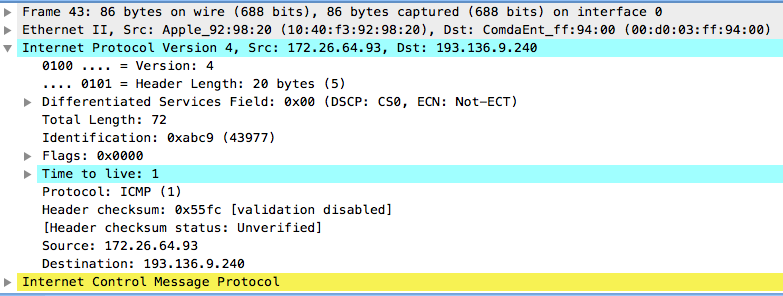
\includegraphics[scale=0.35]{1Pacote} 
\caption{\label{fig:controller}Primeiro Pacote.}
\end{figure} 
\begin{figure}[H]
\centering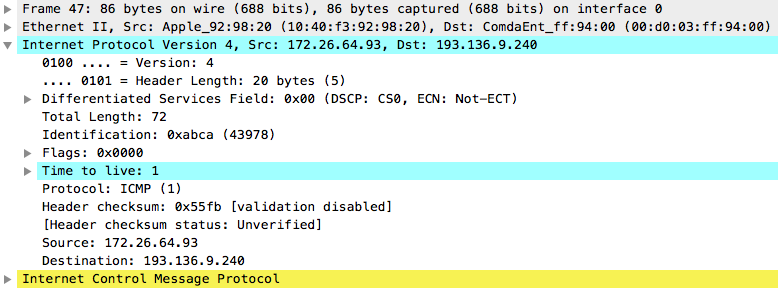
\includegraphics[scale=0.35]{2Pacote} 
\caption{\label{fig:controller}Segundo Pacote.}
\end{figure} 
\begin{figure}[H]
\centering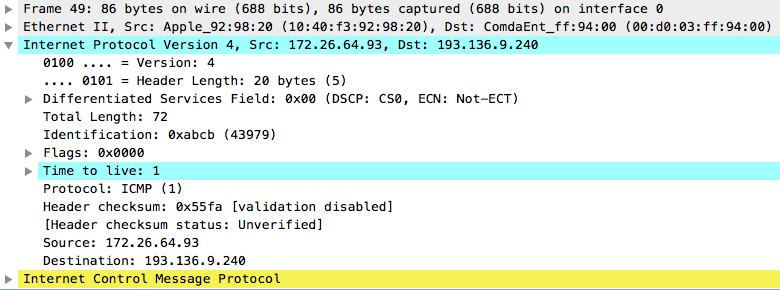
\includegraphics[scale=0.35]{3Pacote} 
\caption{\label{fig:controller}Terceiro Pacote.}
\end{figure} 
\end{solution}

\question Observa algum padrão nos valores do campo de Identificação do datagrama IP e TTL?
\begin{solution}[2in]
Sim. Os valores do campo de Identificação são incrementados em uma unidade por cada pacote enviado e o TTL  é incrementado uma unidade a cada 3 pacotes.
\end{solution}

\question Ordene o tráfego capturado por endereço destino e encontre a série de respostas ICMP TTL exceeded 
enviadas ao seu computador. Qual é o valor do campo TTL? Esse valor permanece constante
para todas as mensagens de resposta ICMP TTL exceeded enviados ao seu host? Porquê?
\begin{solution}[2in]
O valor do campo TTL  é 255, e o mesmo não permanece constante visto que é decrementado em 1 unidade a cada 3 pacotes.
\end{solution}

\end{questions}

\subsection{Exercício 3}

\begin{questions}

\question Localize a primeira mensagem ICMP. Porque é que houve necessidade de fragmentar o pacote inicial?
\begin{solution}[.2in]
Houve a necessidade de fragmentar o pacote inicial pois o mesmo excede o 
Maximum Transmission Unit. O Maximum Transmission Unit  refere-se ao tamanho 
do maior pacote que uma camada de um protocolo de comunicação pode 
transmitir. 
\end{solution}

\question Imprima o primeiro fragmento do datagrama IP segmentado. Que informação no 
cabeçalho indica que o datagrama foi fragmentado? Que informação no 
cabeçalho IP indica que se trata do primeiro fragmento? 
Qual é o tamanho deste datagrama IP?
%PERGUNTAR SE QUEREM O TAMANHO TOTAL DO DATAGRAM OU DO FRAGMENTO??
\begin{solution}[.2in]
As informações do datagrama IP que indicam que o pacote foi fragmentado 
são os respectivos valores que as flags Fragment Offset e More Fragments
tomam, sendo que podemos afirmar que se trata do primeiro fragmento pois 
as mesmas tomam os valores 0 e 1. O tamanho do datagrama é de 3535 bytes.
\begin{figure}[H]
\centering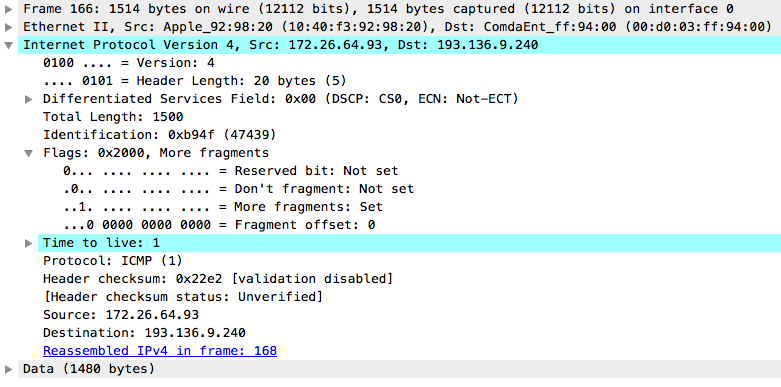
\includegraphics[scale=0.35]{1fragmento} 
\caption{\label{fig:controller}Primeiro Fragmento.}
\end{figure} 
\end{solution}

\question Imprima o segundo fragmento do datagrama IP original. Que 
informação do cabecalho IP indica que não se trata do primeiro fragmento?
Há mais fragmentos? O que nos permite afirmar isso?
\begin{solution}[.2in]
Sabe-se que não se trata do primeiro fragmento devido ao valor da flag 
Fragment Offset , sendo que podemos afirmar que não se trata do primeiro
fragmento pois a mesma toma um valor diferente de 0. Podemos afirmar 
que existem mais fragmentos pois a flag More Fragments tem o valor 1.
\begin{figure}[H]
\centering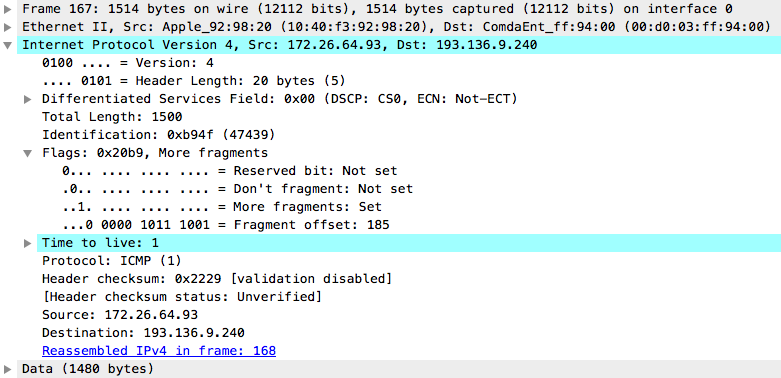
\includegraphics[scale=0.35]{2fragmento} 
\caption{\label{fig:controller}Segundo Fragmento.}
\end{figure} 
\end{solution}

\question Quantos fragmentos foram criados a partir do datagrama original? 
Como se detecta o último fragmento correspondente ao datagrama original?
\begin{solution}[.2in]
A partir do datagrama original foram criados 3 fragmentos, 
tendo cada um o seguinte tamanho:
\begin{description}
	\item[•] \textbf{Primeiro Fragmento:} 1480 bytes.
	\item[•] \textbf{Segundo Fragmento:} 1480 bytes.
	\item[•] \textbf{Último Fragmento:} 575 bytes.
\end{description}	
Podemos ainda detectar o último fragmento através das flags Fragment 
Offset e More Fragments, pois o Fragment Offset terá um valor diferente 
de 0 e a More Fragments será igual a 0, podendo ainda fazer-se a 
verificação de que se trata do mesmo datagrama através do campo 
Identification.
\begin{figure}[H]
\centering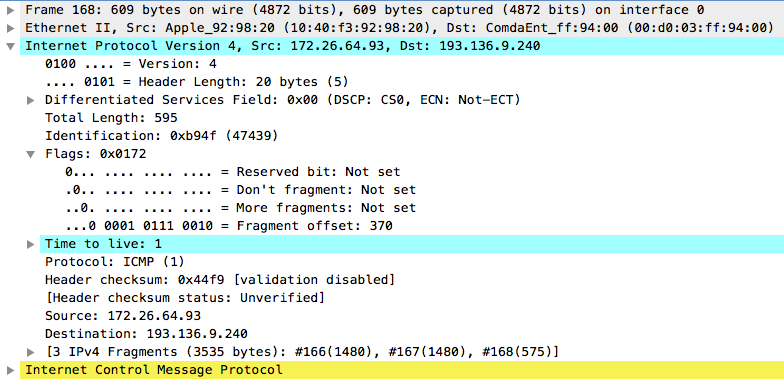
\includegraphics[scale=0.35]{ultimofragmento} 
\caption{\label{fig:controller}Último Fragmento.}
\end{figure} 
\end{solution}

\question Indique, resumindo, os campos que mudam no cabeçalho IP entre 
os diferentes fragmentos, e explique a forma como essa informação permite
reconstruir o datagrama original.

\begin{solution}[.2in]
Os campos que mudam no cabeçalho entre os diferentes fragmentos são:
\begin{description}
	\item[•] \textbf{Flag More Fragments.} 
	\item[•] \textbf{Flag Fragment Offset.}
	\item[•] \textbf{Header Cheksum.}  
\end{description}
Um receptor sabe que um pacote é um fragmento caso a sua flag More Fragments esteja activa (excepto no último fragmento) e caso a
flag Fragment Offset do Fragmento tenha um valor diferente de 0 (excepto para o primeiro fragmento). Os fragmentos que possuirem a mesma identificação
pertecem ao mesmo datagrama, e o campo do Offset do fragmento permite ordenar esses fragmentos.
Ao receber o último fragmento o receptor pode então calcular o tamanho do campo de dados tirando partido da seguinte fórmula:
\begin{equation}
Tamanho Total=Offset*8 + (Total Length-Header Length)
\end{equation}
Sendo que o Offset e o Total Length correspondem a valores do último fragmento. Logo o pacote é remontado no seu destino final e
é enviado para a camada superior concretamente a de Transporte.
\end{solution}
\end{questions}

\section{Parte II}
\subsection{Exercício 1}
\begin{questions}

\question Indique que endereços IP e máscaras de rede foram atribuídas pelo CORE 
a cada equipamento.
\begin{figure}[H]
\centering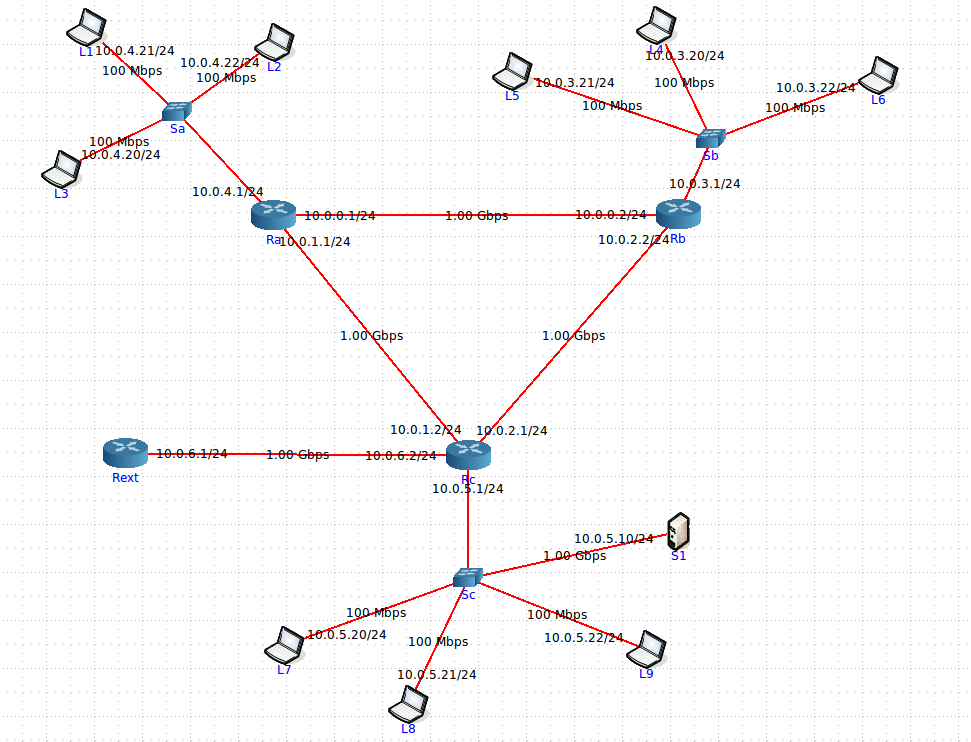
\includegraphics[scale=0.48]{enderecosEmascaras} 
\caption{\label{fig:controller}Endereços IP e máscaras de rede atribuídas pelo CORE.}
\end{figure} 

\question Trata-se de endereços públicos ou privados? Porquê?
\begin{solution}
Tratam-se de endereços privados pois pertencem à gama de valores da classe A: de 10.0.0.0 a 10.255.255.255 (10.0.0.0 /8).
\end{solution}	

\question Porque razão não é atribuído um endereço IP aos switches?
\begin{solution}
Porque os switches trabalham na camada de dados e não têm capacidade para trabalhar na cama de rede IP.
\end{solution}	

\question Certifique-se	que	existe conectividade IP entre os laptops dos vários departamentos e	o servidor do departamento C.
\begin{solution}
\begin{figure}[H]
\centering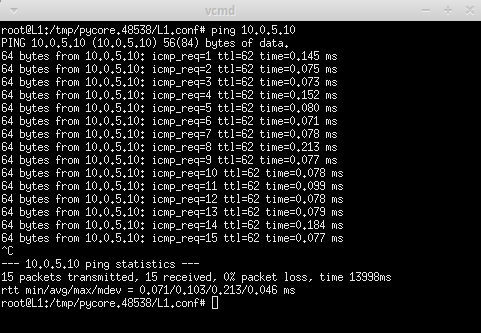
\includegraphics[scale=0.50]{conetividadeA} 
\caption{\label{fig:controller}Conetividade IP entre o laptop L1 e servidor S1.}
\end{figure} 
\begin{figure}[H]
\centering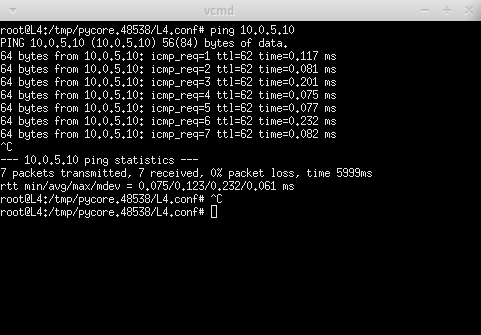
\includegraphics[scale=0.50]{conetividadeB} 
\caption{\label{fig:controller}Conetividade IP entre o laptop L4 e servidor S1.}
\end{figure} 
\begin{figure}[H]
\centering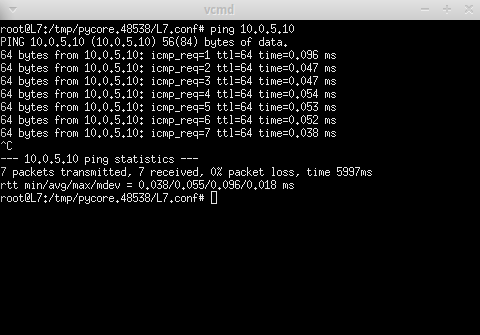
\includegraphics[scale=0.50]{conetividadeC} 
\caption{\label{fig:controller}Conetividade IP entre o laptop L7 e servidor S1.}
\end{figure} 
\end{solution}

\question Certifique-se	que	existe conectividade IP do router de acesso Rext para o servidor S1.
\begin{solution}
\begin{figure}[H]
\centering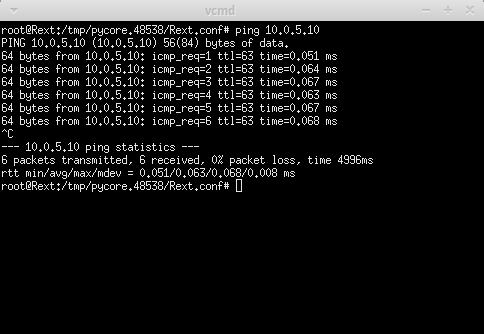
\includegraphics[scale=0.50]{conetividadeRext} 
\caption{\label{fig:controller}Conetividade IP entre Rext e servidor S1.}
\end{figure} 
\end{solution}

\end{questions}

\subsection{Exercício 2}

\begin{questions}

\question Execute o	comando	netstat –rn por	forma a	poder consultar a tabela de	encaminhamento unicast(IPv4).
\begin{solution}
\begin{figure}[H]
\centering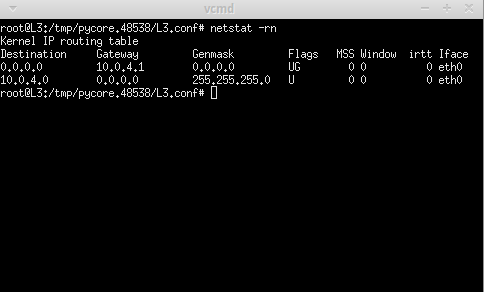
\includegraphics[scale=0.50]{netStatLaptop} 
\caption{\label{fig:controller}Tabela de encaminhamento do laptop L3 do departamento A.}
\end{figure} 
\begin{figure}[H]
\centering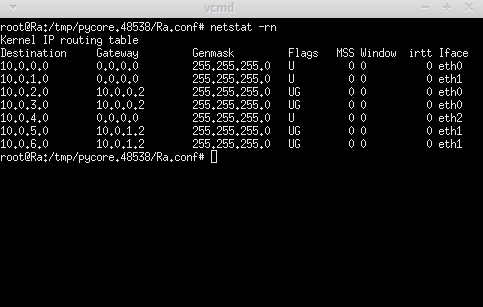
\includegraphics[scale=0.50]{netStatRouter} 
\caption{\label{fig:controller}Tabela de encaminhamento do router do departamento A.}
\end{figure} 
\end{solution}

\question Diga, justificando, se está a ser usado encaminhamento estático ou dinâmico.
\begin{solution}
Laptop: Tirando partido do comando ps -A, podemos verificar que não está a correr nenhum protocolo de encaminhamento 
logo o encaminhamento é estático.
\begin{figure}[H]
\centering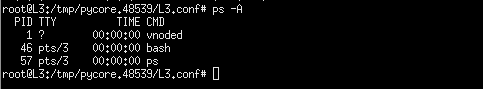
\includegraphics[scale=0.50]{processosAnalise} 
\caption{\label{fig:controller}Processos que correm no laptop L3.}
\end{figure} 
Router: Tirando partido do comando ps- A, podemos verificar que está a correr o protocolo ospfd logo o encaminhamento é
dinâmico.
\begin{figure}[H]
\centering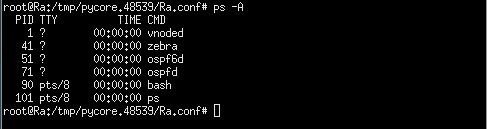
\includegraphics[scale=0.50]{processosAnalise1} 
\caption{\label{fig:controller}Processos que correm no router do departamento A.}
\end{figure} 
\end{solution}

\question Admita que, por questões administrativas, a	rota por defeito(0.0.0.0 ou	
default) deve ser retirada definitivamente da tabela de	encaminhamento	
do servidor S1 localizado no departamento C. Use o comando route
delete para	 o efeito. Que	implicações tem esta medida	para os
utilizadores da	empresa	que acedem ao servidor.	Justifique.
\begin{solution}
Com a remoção da rota por defeito não seria possível enviar ou receber qualquer datagrama no servidor.
\begin{figure}[H]
\centering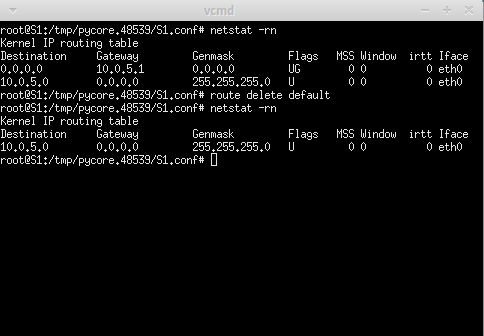
\includegraphics[scale=0.50]{delete} 
\caption{\label{fig:controller}Remoção da rota por defeito.}
\end{figure} 
\end{solution}

\question Adicione as	rotas estáticas	necessárias para restaurar a conectividade	
para o servidor S1. Utilize	para o efeito o	comando	route add e	registe	os comandos que	
usou.
\begin{solution}
\begin{figure}[H]
\centering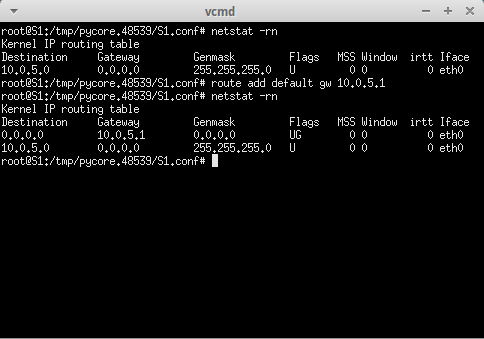
\includegraphics[scale=0.50]{add} 
\caption{\label{fig:controller}Adição da rota estática.}
\end{figure} 
\end{solution}

\question Teste a nova política de encaminhamento garantindo que o servidor está
novamente acessível, utilizando	para o efeito o	comando	ping. 
\begin{solution}
\begin{figure}[H]
\centering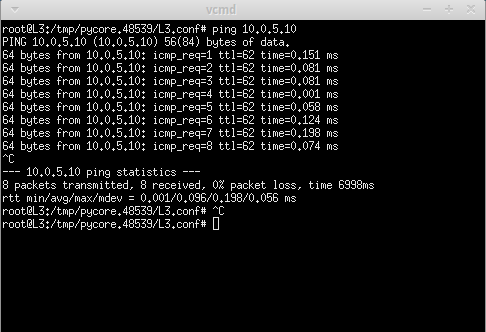
\includegraphics[scale=0.50]{pingL3} 
\caption{\label{fig:controller}Conetividade IP entre laptop L3 e servidor S1.}
\end{figure} 
\begin{figure}[H]
\centering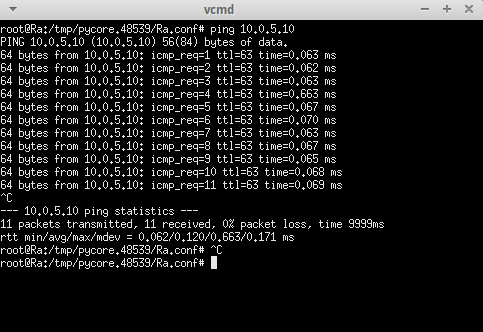
\includegraphics[scale=0.50]{pingRa} 
\caption{\label{fig:controller}Conetividade IP entre Ra e servidor S1.}
\end{figure} 
\end{solution}

\end{questions}

\subsection{Exercício 3}

\begin{questions}

\question Considere que	dispõe apenas do endereço de rede IP 172.XX.48.0/20, em que	XX	
é o	decimal	correspondendo ao seu número de	grupo(PLXX). Defina	um novo	
esquema	de endereçamento para as redes dos departamentos (mantendo a rede	
de acesso e core inalteradas) e	atribua endereços às interfaces dos vários	
sistemas envolvidos.	
\begin{solution}
Sendo que a nossa topologia possuí 3 departamentos para fazer o subnetting seria 
necessário pelo menos 2 bits para as subredes, mas visto que duas 
das quatro opções correspondem a endereços privados só 
seria possível fazer o subnetting a dois dos três 
departamentos. Trabalhando com 3 bits teríamos 
disponível 6 opções válidas para definir as subredes.
Logo teríamos 9 bits reservados para os hosts e 3 bits 
para as subredes.
\end{solution}
\begin{figure}[H]
\centering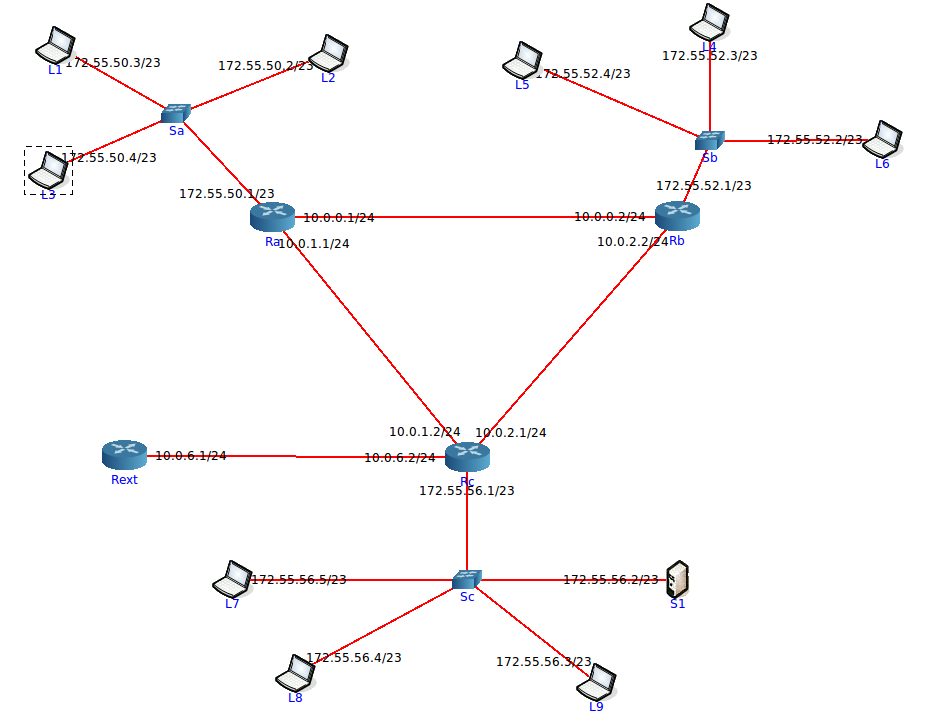
\includegraphics[scale=0.48]{novaRede} 
\caption{\label{fig:controller}Topologia após o subnetting.}
\end{figure} 

\question Qual a máscara de rede que usou(em formato decimal)? Quantos hosts IP pode	
interligar em cada departamento? Justifique.
\begin{solution}
\begin{equation}
Mascara:255.255.254.0
\end{equation}
\begin{equation}
Hosts: 2^9 - 2=510
\end{equation}
\end{solution}

\question Garanta e verifique que conectividade IP entre as várias redes locais da organização
MIEI-RC é mantida. Explique como procedeu.
\begin{solution}
\begin{figure}[H]
\centering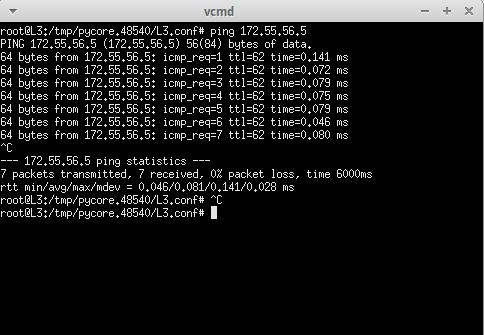
\includegraphics[scale=0.50]{conAeB} 
\caption{\label{fig:controller}Conetividade IP entre departamento A e B.}
\end{figure} 
\begin{figure}[H]
\centering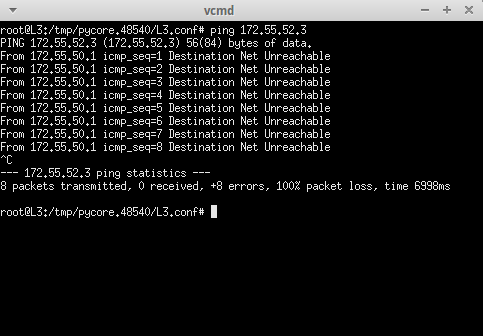
\includegraphics[scale=0.50]{conAec}
\caption{\label{fig:controller}Conetividade IP entre departamento A e C.}
\end{figure} 
\begin{figure}[H]
\centering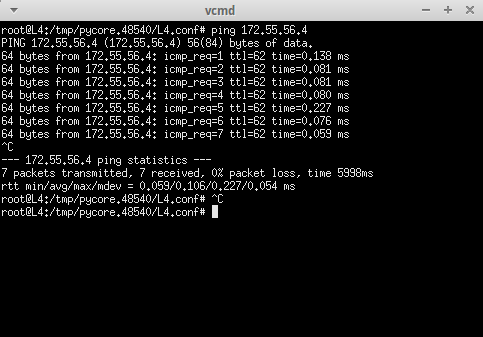
\includegraphics[scale=0.50]{conBeC}
\caption{\label{fig:controller}Conetividade IP entre departamento B e C.}
\end{figure} 
Tirando partido do comando ping conseguimos ver que existe conetividade entre as várias redes locais.
\end{solution}

\end{questions}

\section{Conclusão}
Quanto à primeira parte do TP podemos concluir que:
\begin{itemize}
	\item No envio de datagramas, por forma a impedir que estes sejam reencaminhados indefinidamente, 
	é usado um parâmetro presente no cabeçalho IP designado TTL, que limita o número de \textit{hop's}. 
	Desta forma, para que um datagrama seja entregue num destino a N \textit{hop's} de distância, 
	é necessário que o TTL tenha um valor mínimo de N.
	\item Quando o tamanho dos datagramas excede a MTU é necessário recorrer a um processo designado 
	de fragmentação que consiste em dividir os datagramas em partes mais pequenas(fragmentos) que são 
	reassemblados no destino recorrendo a flags como: \textit{Fragment Offset} e \textit{More Fragments}.
\end{itemize}

Relativamente à segunda parte do TP, concluímos que os \textit{hosts/end systems} não mantêm 
tabelas de encaminhamento extensas, visto que a maioria do tráfego é encaminhado para o 
\textit{router}, sendo que estes últimos recorrem a protocolos de routeamento(OSPF, RIP, etc) 
para determinar as melhores rotas para um determinado destino. Por outro lado, e por forma a 
limitar o tamanho das tabelas, o encaminhamento é feito salto a salto i.e. o \textit{router} 
apenas se preocupa com o próximo \textit{hop}.

\end{document}